\chapter{Testing \& Success Measurement}\label{sec:Testing}
In order to measure the degree of success a project achieves, testing must be performed to verify the behaviour of the program is correct.
This covers testing the functionality of individual units of the program (unit testing), testing how those units interact with each other (integration testing), and validating the behaviour of the overall system against the functional and non-functional requirements\todocite{https://reqtest.com/testing-blog/different-levels-of-testing/}.
This section also defines the means of Success Measurement for some non-functional requirements, which are then measured and evaluated in subsequent sections.% The codebase does not lend itself well to automatic testing, as most components have behaviour that's too difficult to automatically verify (such as automatic memory management, or the entire visualization).
% \todomark{More on explanation of Testing chapter}

\section{Unit Tests}
The first layer of testing splits the program into `units', that are independent of each other, which are individually tested before combining them with other units in the system.
In some systems it is practical to automate these tests, but this was not pursued for this system as the behaviour is generally too complex to be automatically verified.

Helpfully the program is already split into subcommands at the command-line level (\cref{sec:DesignSubcommands}), which can all be tested individually.
% The \texttt{compare}, \texttt{renderppm}, and \texttt{fixedtime} subcommands can each be tested completely independently of other.
Because the file format is the same as the original coursework, the original input file can be used to test comparisons (\texttt{compare}), simple visualization (\texttt{renderppm}), and both simulations (\texttt{fixedtime} and \texttt{run}).
These commands all have equivalents in the original coursework, which provides a basis for validating correctness.
The \texttt{makeinput} subcommand, which creates a new input file based on an image, can be tested by passing the resulting input file to other known-functional subcommands and checking their behaviour.
This provides a coarse view of system functionality, but a finer level of detail can be obtained by testing individual code components.

Unit-testing this particular codebase is difficult because many components are dependent on other components - for example, the visualization components use data gathered from the simulation output, which is impractical to extract for the sake of testing individual components.
It is easier to just test the complete visualized simulation while assuming the simulation itself is correct.
In other cases, unit behaviour may be impractical to directly model or verify: the automated resource management classes are difficult to test individually as the creation/destruction of the resources they manage cannot be directly checked.
However there are some areas where the codebase can be effectively unitized, the most prominent of which is the simulation itself.

The simulation is split into stages, which are effectively independent code units.
Each unit depends on the output of the previous unit, so they cannot be tested independently, but if the rest of the simulation units are known to be correct then an individual unit can be tested.
This technique was used during development to ensure the CUDA simulation was consistent with the CPU version.

Overall, while unit tests are not always suitable for elements of the codebase, they are helpful at a coarse level.
The final set of unit tests are shown in \cref{tab:unittests}.

\section{Integration Testing}
Once the program units have been individually tested, Integration Testing tests if the units can interface with each other correctly.
Again the subcommands are treated as units, and testing is performed by passing an output from one subcommand as the input to another.
In this program only the \texttt{makeinput} and \texttt{fixedtime} subcommands produce output, so their output is exhaustively tested against the other commands.
At the codebase level some previous unit tests can be counted as integration tests:
the headless simulation functions as an integration test for the Memory and Simulation layers, and the visualized simulation tests the integration between the Simulation and Visualization layers.

The C++ type system ensures that low-level connections between CPU code use the correct types, making integration testing at this level redundant.
Moving data between the CPU and GPU is more complicated, but the elements put in place in (\cref{sec:Impl:Viz:CPUGPUSafety}) and the Vulkan validation layers (\cref{sec:Impl:CodeSafety}) ensure that any integration errors are caught when simply running the program in Debug mode.

The Integration tests are shown in \cref{tab:integration_tests}.



\section{System Testing}
This final layer of testing determines if the program upholds the functional and non-functional requirements set out in \cref{sec:Requirements}.
Some functional requirements such as \cref{req:VizPauseResume} require in-depth checks of the visualization not suitable for other layers, so are tested here.
The System Tests specified in \cref{tab:sys_tests_func} cover all such tests, and combined with the previous layers of tests prove that the system meets the functional requirements.

Many non-functional requirements can be tested directly: \cref{reqN:Resources} is tested with external programs \texttt{valgrind} and \texttt{cuda-memcheck}, \cref{reqN:Documented,reqN:UsageGuide} are tested by simply inspecting the program and source files, \cref{reqN:DCSCompile} is tested by attempting to compile + run the program on DCS systems.
A few require a large amount of data collection, or at least careful attention to detail.
% The others need special care and extra specification to measure qualitatively.
% The nonfunctional tests (\todoref{system tests nonfunctional}) handle the non-functional requirements.
% Some of these tests are more complex and require more data to evaluate them.
These tests are specified in \cref{tab:sys_tests_nonfunc}.
All gathered data is specified in the next subsection, and then the results are shown in \cref{sec:Results}.

% \newcommand{\testsuccess}{\symbol{"2B45}}
% \newcommand{\testfail}{\symbol{"2718}}

\newcommand{\testsuccess}{\cmark{}}
\newcommand{\testfail}{\xmark{}}

% \pagebreak
% \newgeometry{margin=2cm}
% \begin{sidewaysfigure}
%     \centering
%     \makebox[\linewidth][c]{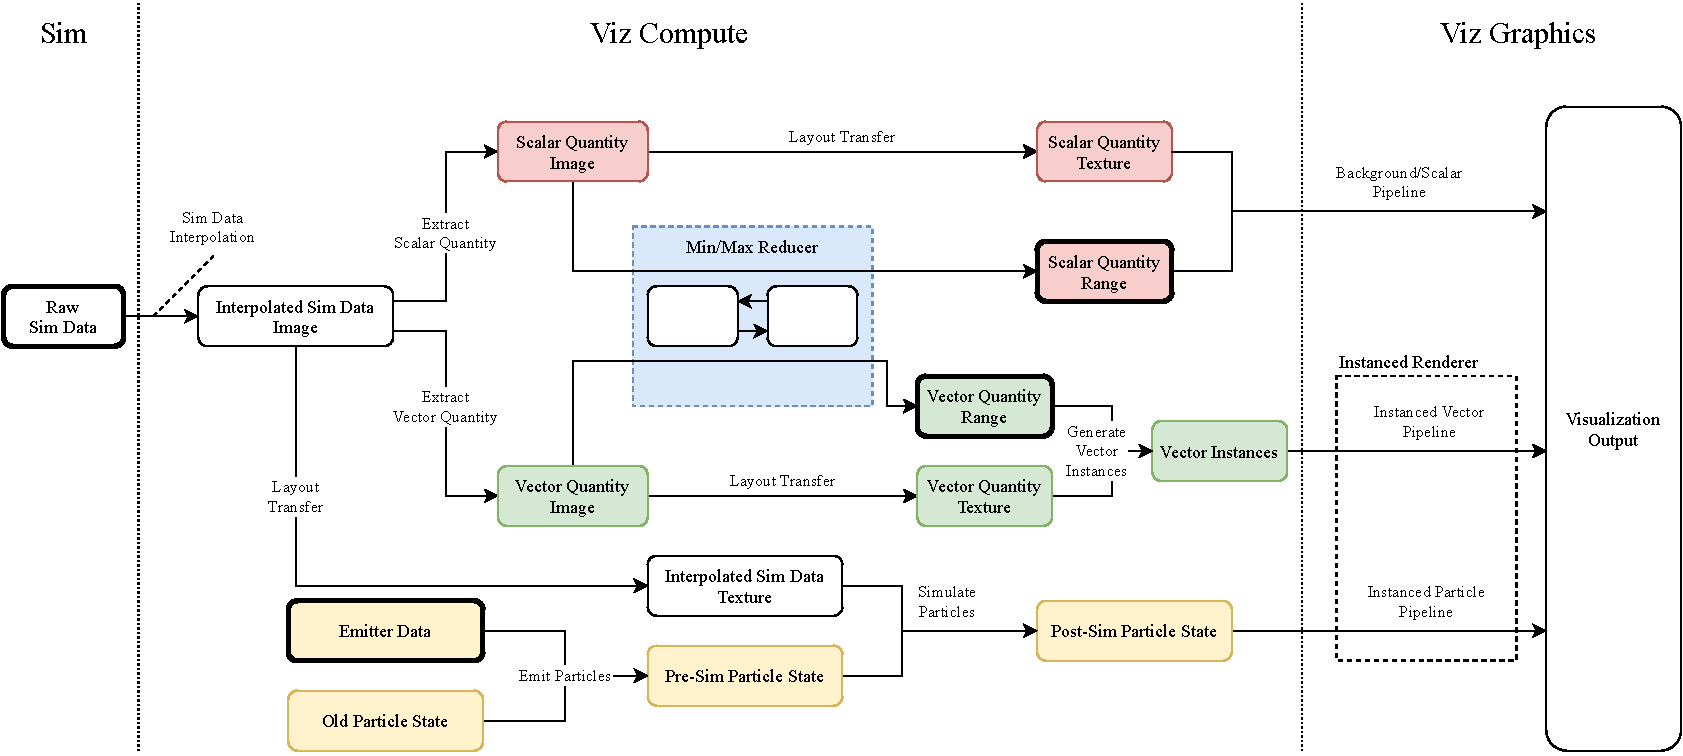
\includegraphics[width=\linewidth]{Ch48Implementation/figures/FinalReport_VizData.pdf}}
%     \caption{Data Transformation Diagram showing the data flow for the Visualization}
%     \label{fig:VizDataTransform}
% \end{sidewaysfigure}
% \restoregeometry
% \pagebreak

\begin{sidewaystable}
    \centering
    \begin{tabular}{ll|c|c|c}
        ID & Description & Expected & Output & Result \\
        \hline
        \newtest{}\label{test:unit:compare:identical} & \shell{compare}: identical states & No difference & No difference & \testsuccess{} \\
        \newtest{}\label{test:unit:compare:different} & \shell{compare}: Original input to original target output & Some difference & Some difference & \testsuccess{} \\
        \newtest{}\label{test:unit:renderppm} & \shell{renderppm}: render state vorticity & Equal to original program & Equal to original program & \testsuccess{} \\
        \newtest{}\label{test:unit:makeinput} & \shell{makeinput}: generate an input file from a PNG & Valid simulation state & Valid simulation state & \testsuccess{} \\
        \newtest{}\label{test:unit:fixedtime} & \shell{fixedtime}: simulate from an input state for 25 seconds. & Valid simulation state & Valid simulation state & \testsuccess{} \\
        \newtest{}\label{test:unit:run} & \shell{run}: visualize a simulation from an input state for 25 seconds. & Valid simulation state & Valid simulation state & \testsuccess{} \\
    \end{tabular}
    \caption{Unit Tests}
    \label{tab:unittests}
\end{sidewaystable}


\newcommand{\integtest}[2]{\shell{#1} & $\xrightarrow{}$ & \shell{#2}}
\newcommand{\successoutput}[1]{#1 & As expected & \testsuccess{}}

\begin{sidewaystable}
    \centering
    \begin{tabular}{lccl|p{0.4\linewidth}|m{0.2\linewidth}|c}
        ID & \multicolumn{3}{l}{Integrated Modules} & Expected & Output & Result \\
        \hline
        \newtest{}\label{test:intg:input:render} & \integtest{makeinput}{renderppm} & \successoutput{Valid render image with the same obstacle squares as the initial image.} \\
        \newtest{}\label{test:intg:input:cmp} & \integtest{makeinput}{compare} & \shell{compare} runs successfully & \shell{compare} ran successfully & \testsuccess{} \\
        \newtest{}\label{test:intg:input:sim} & \integtest{makeinput}{fixedtime} & \successoutput{Valid simulation output with the same obstacle squares as the initial image.} \\
        \newtest{}\label{test:intg:input:viz} & \integtest{makeinput}{run} & \successoutput{Visualization of a simulation with the same obstacle squares as the initial image.} \\
        \hline
        \newtest{}\label{test:intg:sim:render} & \integtest{fixedtime}{renderppm} & \successoutput{Valid render image with the same obstacle squares as the initial state.} \\
        \newtest{}\label{test:intg:sim:cmp} & \integtest{fixedtime}{compare} & \shell{compare} runs successfully & \shell{compare} ran successfully & \testsuccess{} \\
        \newtest{}\label{test:intg:sim:sim} & \integtest{fixedtime}{fixedtime} & \successoutput{Valid simulation output with the same obstacle squares as the initial state.} \\
        \newtest{}\label{test:intg:sim:viz} & \integtest{fixedtime}{run} & \successoutput{Visualization of a simulation with the same obstacle squares as the initial state.} \\
    \end{tabular}
    \caption{Integration Tests}
    \label{tab:integration_tests}
\end{sidewaystable}

\begin{sidewaystable}
    \centering
    \begin{tabular}{ll|p{0.35\linewidth}|m{0.2\linewidth}|c}
        ID & Description & Expected & Output & Result \\
        \hline
        \newtest{}\label{test:sys:sim:gpu} & \texttt{fixedtime}: GPU Simulation & \successoutput{Simulation backend can be set to CUDA} \\
        \newtest{}\label{test:sys:run:gpu} & \texttt{run}: GPU Simulation & \successoutput{Simulation backend can be set to CUDA} \\%Can visualize a simulation running on the GPU
        \hline
        \newtest{}\label{test:sys:run:pause} & \texttt{run}: Test pausing/resuming the simulation & \successoutput{Simulation can pause/resume while the visualization is running} \\
        \newtest{}\label{test:sys:run:save} & \texttt{run}: Test saving the simulation state & Simulation state can be saved while visualizing & Couldn't save state while running & \testfail{} \\
        \newtest{}\label{test:sys:run:manip} & \texttt{run}: Test moving the particle emitters & \successoutput{Particle emitters can be moved while the simulation is running} \\
        \newtest{}\label{test:sys:run:lockedFPS} & \texttt{run}: Can run with a fixed framerate & Framerate can be fixed at some value & Framerate was fixed at 120FPS and did not change & \testsuccess{} \\
        \newtest{}\label{test:sys:run:flatoutFPS} & \texttt{run}: Can run with an unlocked framerate & Framerate can be unlocked & Framerate was not locked and varied between 750-800FPS & \testsuccess{} \\
        \newtest{}\label{test:sys:run:layerPerms} & \texttt{run}: All Viz layers work as expected. & \successoutput{All layer combinations can be used, all layers function as described in \cref{sec:Requirements}.} \\
        \newtest{}\label{test:sys:run:autorange} & \texttt{run}: Test auto-range functionality & \successoutput{Auto-ranged Scalar and Vector quantities display all values in the sim boundary.} \\
        \newtest{}\label{test:sys:run:colors} & \texttt{run}: Test changing colors & \successoutput{All colors used in the simulation should be modifiable} \\
        \newtest{}\label{test:sys:run:validation} & \texttt{run}: Check Vulkan validation & \successoutput{No Vulkan validation errors in Debug mode} \\
    \end{tabular}
    \caption{System Tests (Functional)}
    \label{tab:sys_tests_func}
\end{sidewaystable}

\begin{sidewaystable}
    \centering
    \begin{tabular}{lp{0.2\linewidth}|p{0.4\linewidth}|m{0.2\linewidth}|c}
        ID & Description & Expected & Output & Result \\
        \hline
        \newtest{}\label{test:sys:sim:large} & \texttt{run}: Large Simulation & \successoutput{Simulation can run on a 4096x4096 input.} \\
        \newtest{}\label{test:sys:sim:valgrind} & \texttt{run}: No CPU memory leaks & Visualization run under \texttt{valgrind} should have no program-controlled memory leaks. & See \cref{sec:Results:Sim:Mem,sec:Results:Viz:Memory} & \testsuccess{} \\
        \newtest{}\label{test:sys:sim:cudamemcheck} & \texttt{run}: No CUDA memory leaks & Simulation run under \texttt{cuda-memcheck} should have no program-controlled memory leaks. & See \cref{sec:Results:Sim:Mem,sec:Results:Viz:Memory} & \testsuccess{} \\
        \newtest{}\label{test:sys:run:pipeline} & \texttt{run}: High GPU Utilization & Nsight Systems profiler output should show maximum achievable GPU utilization\footnote{100\% may not be possible due to other programs using the GPU} & See \cref{sec:Results:Sim:Efficiency,sec:Results:Viz:Efficiency} & \testsuccess{} \\
        
        
        \newtest{}\label{test:sys:sim:speed} & \texttt{fixedtime}: Simulation is faster than original simulation & CUDA simulation should run 2x faster than the original simulation on the original input. &See \cref{sec:Results:Sim:Speed} & \testsuccess{} \\
        \newtest{}\label{test:sys:sim:accuracy} & \texttt{fixedtime}: Simulation produces similar results to original simulation &
        CUDA simulation solver residual should be within 5\% of adapted CPU backend.
        & See \cref{sec:Results:Sim:Accuracy} & \testsuccess{} \\
        % CUDA simulation output should be within $10^-10$ of the adapted CPU backend output. & See \cref{sec:Results:Sim:Accuracy} & \testfail{} \\

        \newtest{}\label{test:sys:run:highFPS} & \texttt{run}: Can run at high framerate & Visualization can run at >30FPS in some case & Simulating the original input at N=100 runs at \~800FPS. & \testsuccess{} \\
        \newtest{}\label{test:sys:run:vizSpeed} & \texttt{run}: Visualization features are faster than simulation & See \cref{sec:Testing:SuccessMeasurement} & See \cref{sec:Results:Viz:Speed} & \testsuccess{} \\
        \newtest{}\label{test:sys:run:dcsComp} & Try to compile on DCS systems & Should be able to compile and run the simulation on elements of the DCS system. & Successfully compiled non-CUDA sim on DCS. & \testsuccess{} \\
    \end{tabular}
    \caption{System Tests (Non-Functional)}
    \label{tab:sys_tests_nonfunc}
\end{sidewaystable}


\subsection{Success Measurement}\label{sec:Testing:SuccessMeasurement}
\cref{test:sys:sim:valgrind,test:sys:sim:cudamemcheck} test the memory usage of the system.
The most important kind of error they can detect are memory leaks, where memory is allocated without being released, leading to the program taking up memory it does not need anymore.
While it is important to avoid memory leaks in all cases the most important variation is continuous memory leaks, where memory is continuously leaked over and over, or large leaks of sizes larger than 100MB.
Single small leaks are less concerning, as they should not impact the rest of the system greatly.
The programs used to find these leaks may themselves be bad at recognizing allocation/freeing\cite{ValgrindProblemsBlog}, and lead to false-positives.
Care must be taken when evaluating their results.
\cref{test:sys:sim:speed,test:sys:sim:accuracy} evaluate the speed and accuracy of the CUDA-based simulation backend vs. the adapted CPU backend.
The accuracy is measured by comparing the output of equivalent simulations on the original CS257 input state.
Other states were tested, but any newly generated states with obstacles proved to be unstable and produce Not-a-Number outputs on both backends.
The simulation speed is tested on the original CS257 input state, then behaviour at scale is tested on custom generated states with no obstacles.
Obstacle configuration does not affect time-per-tick, so time-per-tick will be a representative value and equal for any state of the same size.
This would not be suitable for accuracy tests, as having no obstacles greatly reduces the complexity and would likely produce disproportionately high accuracy values.

As there is no visual component to the simulation tests, the program is run from a terminal without running the X windowing system.
Combined these tests should give a complete picture of how the CUDA simulation's speed and accuracy will scale, and be enough to evaluate the requirements in context.

% To account for all possible factors, results were gathered for many permutations of variables. \todomark{(shown in variable table?)}
% Two input files are used: the original ACA input file (660x120), and a custom 1024x512 image representing \SI{128}{\metre}x\SI{64}{\metre}s of physical space (see \todoref{figure of circles}).
% Larger images are less likely to fit in cache, so accentuate the impact of memory usage on the algorithm.
% Four different simulation configurations are used, which only differ in Poisson iteration count: 100 (matching the original), 200, 300, and 1000.
% Higher iteration counts ensure the Poisson stage dominates the time taken.
% Each permutation is then run for simulations of 10, 25, and 50 seconds to determine the impact of longer simulations on accuracy.
% To measure the time taken for each test five measurements are taken, the fastest and slowest times are removed, and the three remaining results are then averaged.
% The similarity between tests on different backends is measured using the \texttt{compare} tool, and the Poisson residual for each output is found with a small utility that computes the Poisson RHS (see \cref{sec:Research:SimulationTick}) then immediately determines the residual using the CPU backend.


\cref{test:sys:run:vizSpeed} evaluates the speed of individual visualization features vs. the simulation.
As the time taken to run a simulation tick can be variable based on the input, these visualization speeds are compared to the time allotted to the target 60FPS, i.e. \SI{16.6}{\milli\second}.
These visualization times are measured using the frame-time counter in the GUI (\todoref{example of GUI?}), which measures the average time taken to present the last 32 frames.
First, the time taken to render a frame with no visualization features is taken.
Each feature is then individually enabled, brought to the worst-case scenario (using auto-range where applicable, and rendering the maximum amount of instances where applicable), then the average frame-time is taken.
To ensure the results are not affected by external sources, the program is run in unlocked framerate mode with no other programs running on the system.
This is also the case for the GPU utilization test (\cref{test:sys:run:pipeline}).

These results are shown in \cref{sec:Results}, and then evaluated along with the rest of the test outcomes in \cref{sec:Evaluation}.